\scanpage{99}
% archive sheet number: 101

\uline{Résumé}\quad Cas $E_a$ :

\[
\left|\begin{aligned}
&\text{base}\quad u=e_0,\ v=e_1\\
&\text{forme}\quad\deleted{Q(e_0)=Q(e_1)}\quad Q(xe_0+ye_1)=x^2+ay^2
\end{aligned}\right.
\]

Si on veut \deleted{\unsure{l'on|la}} faire $Q$ sous forme ``\unsure{standart|standard}'', on prend la \inserted{nouvelle} base $\underbrace{e_0}_{1},\underbrace{\frac{1}{\sqrt a}e_1}_{i}$, on trouve donc la base $1,\sqrt a\,i$ d'où

\[
\boxed{\tau=\sqrt a\,i}.
\]

Cas $E'_a$ : base $u,v$, \deleted{\unsure{$e_0,e_1$ étant les|les $e$ étant les|$e_0$, $v=$}} \inserted{\unsure{forme|formes}} distingués p. r. à la base

\[
\begin{aligned}
&e_0=u,\ e_1=2v-u\,;\qquad Q(xe_0+ye_1)=x^2+ay^2\\
&v=\tfrac12(e_0+e_1):
\end{aligned}
\]

on \deleted{\unsure{passe encore|passe encore une}} change encore de base $\underbrace{e_0}_{1},\underbrace{\frac{1}{\sqrt a}e_1}_{\unsure{i|v}}$ base orthonormale et on a $u\Rightarrow1,\ v\longmapsto\frac12(1+\sqrt a\,i)$, donc

\[
\boxed{\tau=\frac12(1+\sqrt a\,i)}=\frac12+\frac{\sqrt a}{2}i
\]

\figure{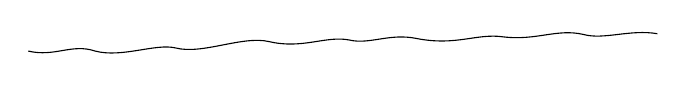
\begin{tikzpicture}[x=.85cm,y=1cm]\draw (0,0) .. controls (.4,-.08) and (.65,.10) .. (1,0) .. controls (1.4,-.09) and (1.9,.1) .. (2.2,.04) .. controls (2.6,-.05) and (3.2,.20) .. (3.6,.12) .. controls (4.1,.02) and (4.45,.20) .. (4.8,.14) .. controls (5.1,.08) and (5.4,.23) .. (5.8,.16) .. controls (6.4,.06) and (6.7,.23) .. (7.1,.18) .. controls (7.6,.13) and (7.9,.29) .. (8.3,.21) .. controls (8.6,.14) and (9,.28) .. (9.4,.22);\end{tikzpicture}}

Calcul \unsure{du groupe|des groupes} des pts réels d'une courbe $E_a,E'_a$.

Pts réels sont les : $x\bmod\pi$ ($x\in\pi_{\mathbb R}$) tels que

\[
\sigma x\equiv x\quad(\pi)
\]

\uline{Distinguons les deux cas}. 1) \uline{$E_a$}\quad $\deleted{\sigma(e_0,e_1)=}\ \sigma(x,y)=x,-y$

\[
\text{donc}\qquad \sigma(x,y)-(x,y)=(0,2y)
\]

donc la condition est que $2y\in\mathbb Z$. Donc il y a \deleted{\unsure{outre|out|ou}} les pts de \deleted{$\unsure{0,\frac12|0,\frac12e|0,}$} $\mathbb R e_0$ et de \deleted{$\unsure{\mathbb R|R_1}$} $(\unsure{0|b},\tfrac12)+\mathbb R e_0$, donc \uline{deux composantes} \uline{connexes} \uline{pour} $X(\mathbb R)$.
